\documentclass[12pt,a4paper]{article}
%\usepackage{xcolor} \pagecolor[rgb]{0.5,0.5,0.5} \color[rgb]{1,1,1}
%\usepackage[utf8]{inputenc}
\usepackage[shortlabels]{enumitem}
%\usepackage{bm}
\usepackage{mathrsfs}
\usepackage{amsmath}
\usepackage{amssymb}
\usepackage{hyperref}
\usepackage{graphicx}
\begin{document}
\title{Solutions to BDA Assignment 2,
 2020/2021 Semester 2}
\author{Theodore Ladas, s2124289}
\date{\today}
\maketitle

This report contains the results from the exploration and modeling of two distrinct statistical problems. The first problem is about modeling the number of earthquakes in Scotland, between 1900 and 2020 from a list of various covariates. 

\noindent\textbf{1)}
\begin{enumerate}[(a)]
\item
Explanation: In this part, an explanatory data analysis is being conducted, in order to gain some initial insight on the dataset. Afterwards, it is assumed that number of earthquakes in Scotland comes from a Poisson distribution with unknown mean parameter $\mu_i$   which is proportional to the number of nonScot earthquakes, namely, 
$\mu_i=\lambda * eartrUK_i$, with the default log link. 

Results:
On \autoref{EDA1} we see a correlation plot, as well as three regressions. On the correlation plot, some things are expected, for example there is a large negative linear correlation between the earthquakes in Scotland \textit{dist} variable, which represents the distance (in miles) of the nearest "nonScot" earthquake to the Scottish border. However we also see a similarly large correalation with decade, indicating that there are less eathquakes in Scotland today, which can be explored further. Lastly, we can also see some problematic regression coefficients between the variables \textit{nrUK4.5}, the number of "nonScot" earthquakes with a magnitude (ML) greater or equal 4.5 and \textit{MLrUK} the average magnitude of "nonScot" earthquakes with $MLrUK > 4$. This suggests that a default logistic regression problem where both of these covariates are present, will have to be very carefully interpreted because of the multicolinearity between those two variables. 

\begin{figure}[h]
    \centering
    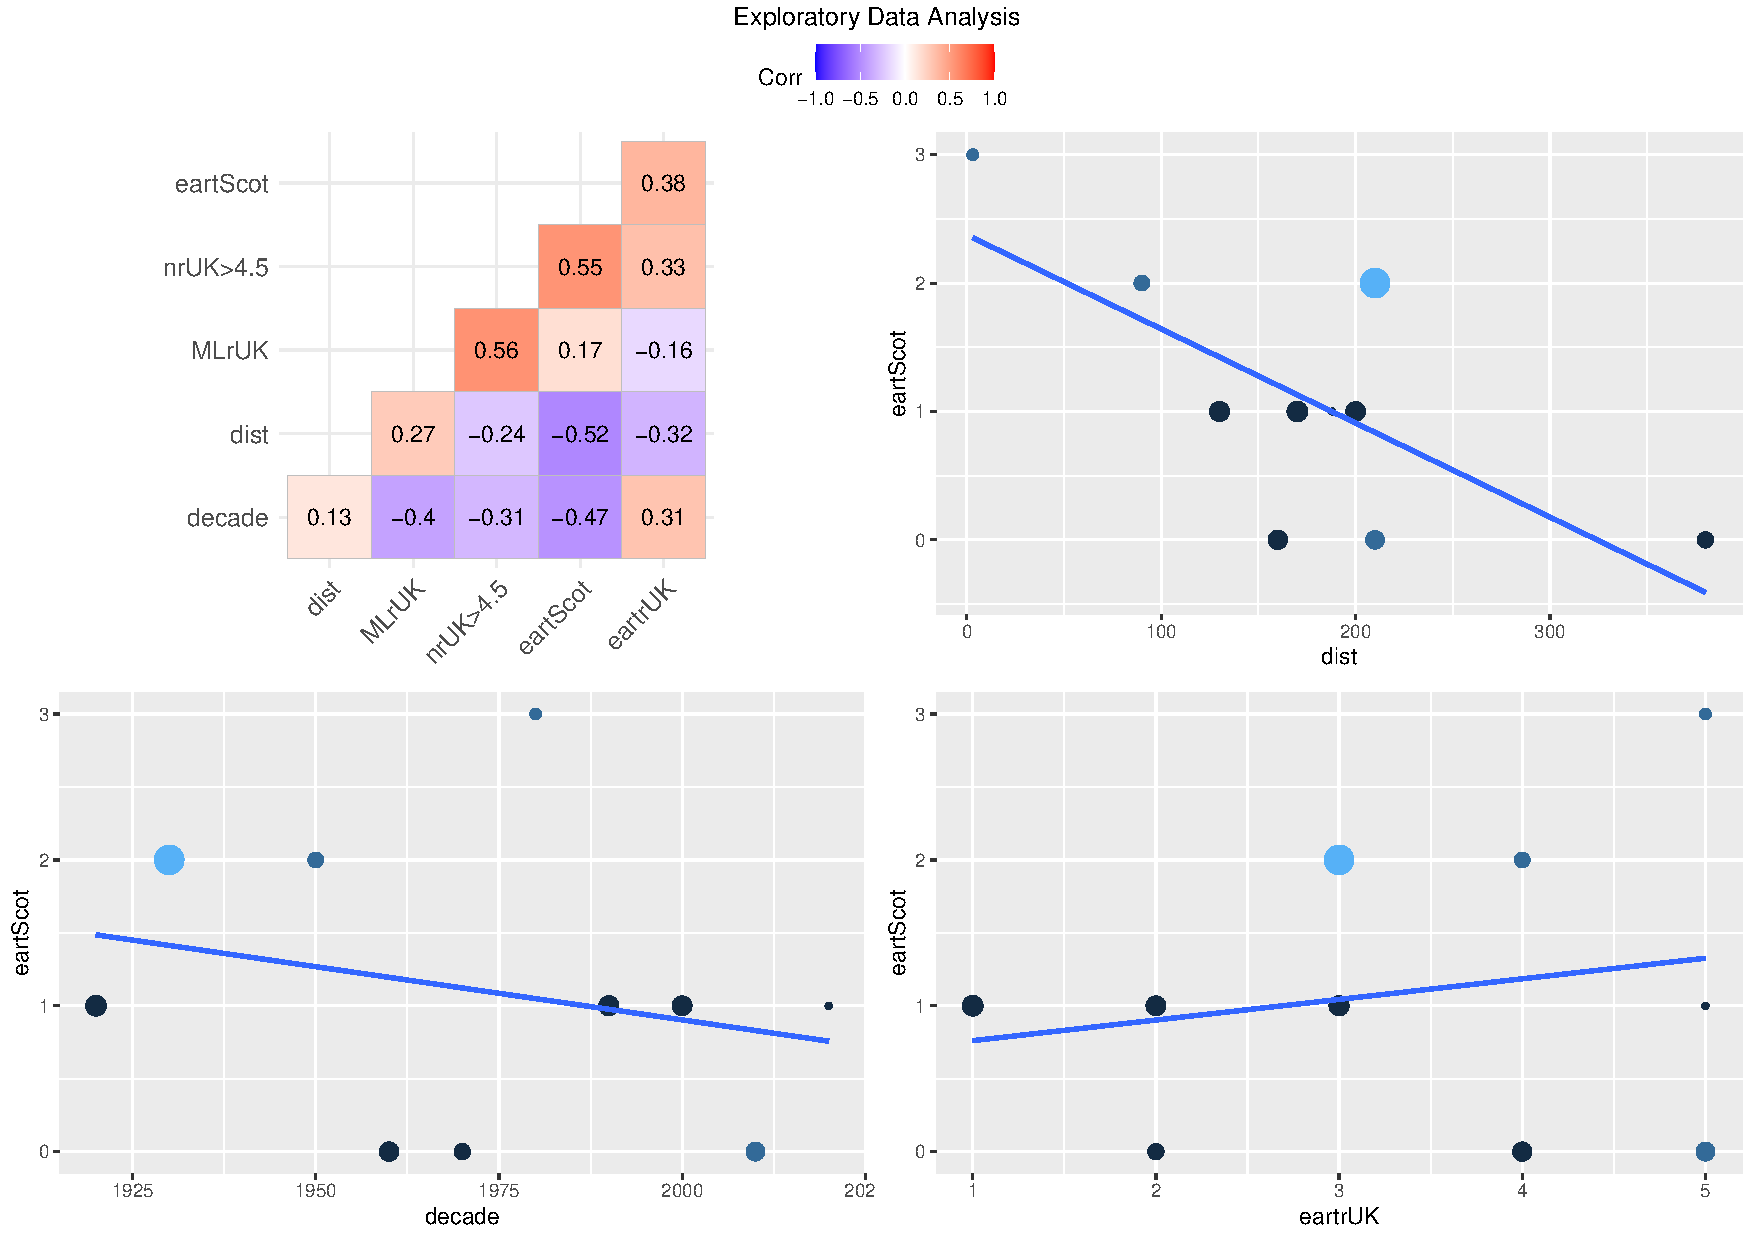
\includegraphics[width=0.7\linewidth]{figures/Rplot00.pdf}
    \caption{EDA}
    \label{EDA1}
\end{figure}

On the rest three diagrams, the magnitude of the eathquake is represented by the size of the dots, while the variable \textit{nrUK4.5} is represented by the colour of the dots. There are too few datapoints in order to accurately estimate the relationship between each covariate and the target variable. For example, we see a very pronounce negative slope on the diagram between \textit{dist} and \textit{eartScot}, but it this could be caused by the outliers on the $0$ and the $>300$ distance from the Scottish boarder. 

TODO: GENERATE ANOTHER PLOT WITH EARTHUK

All in all the exploratory data analysis yields that there is no clear answer as to what variables are useful, although it is hinted that the variable \textit{eartrUK} could be a logical choice.


\begin{figure}[]
    \centering
    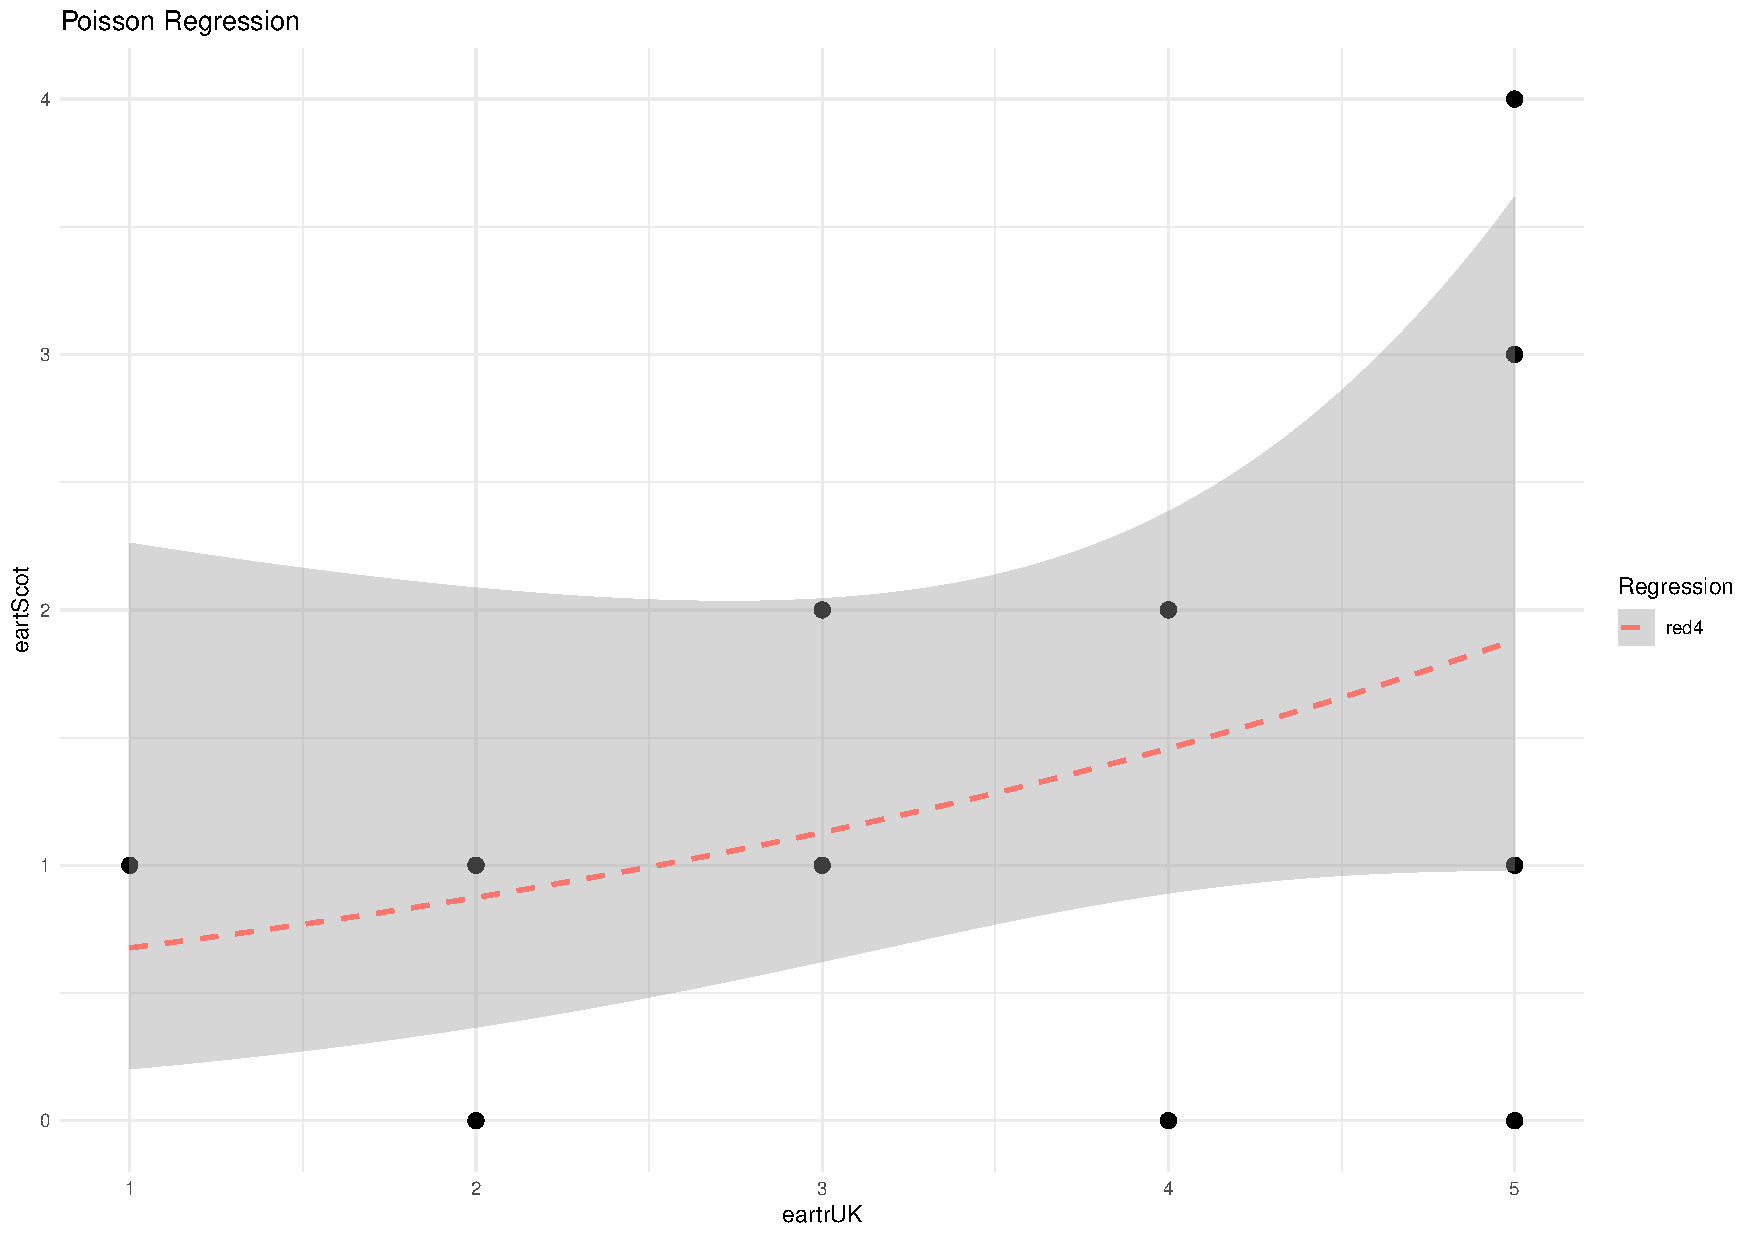
\includegraphics[width=0.6\linewidth]{figures/Rplot01.pdf}
    \caption{Fitted model}
    \label{model1}
\end{figure}

In this section, the results from the logistic regression model are presented. The intercept  of the regression, after unlinking it by using the inverse of the link function (exponentiating) is 0.5238674, while the coefficient of \textit{eartrUK} is 1.2915168. With these coefficients, the expected number of earthquakew in Scotland in the decade of 1970 and in the decade of 1980 are 0.873819 and 1.882442 respectively, where if we round to the nearghrest integer means that there will be 1 and 2 earthquakes in these decades. 

\begin{figure}[]
    \centering
    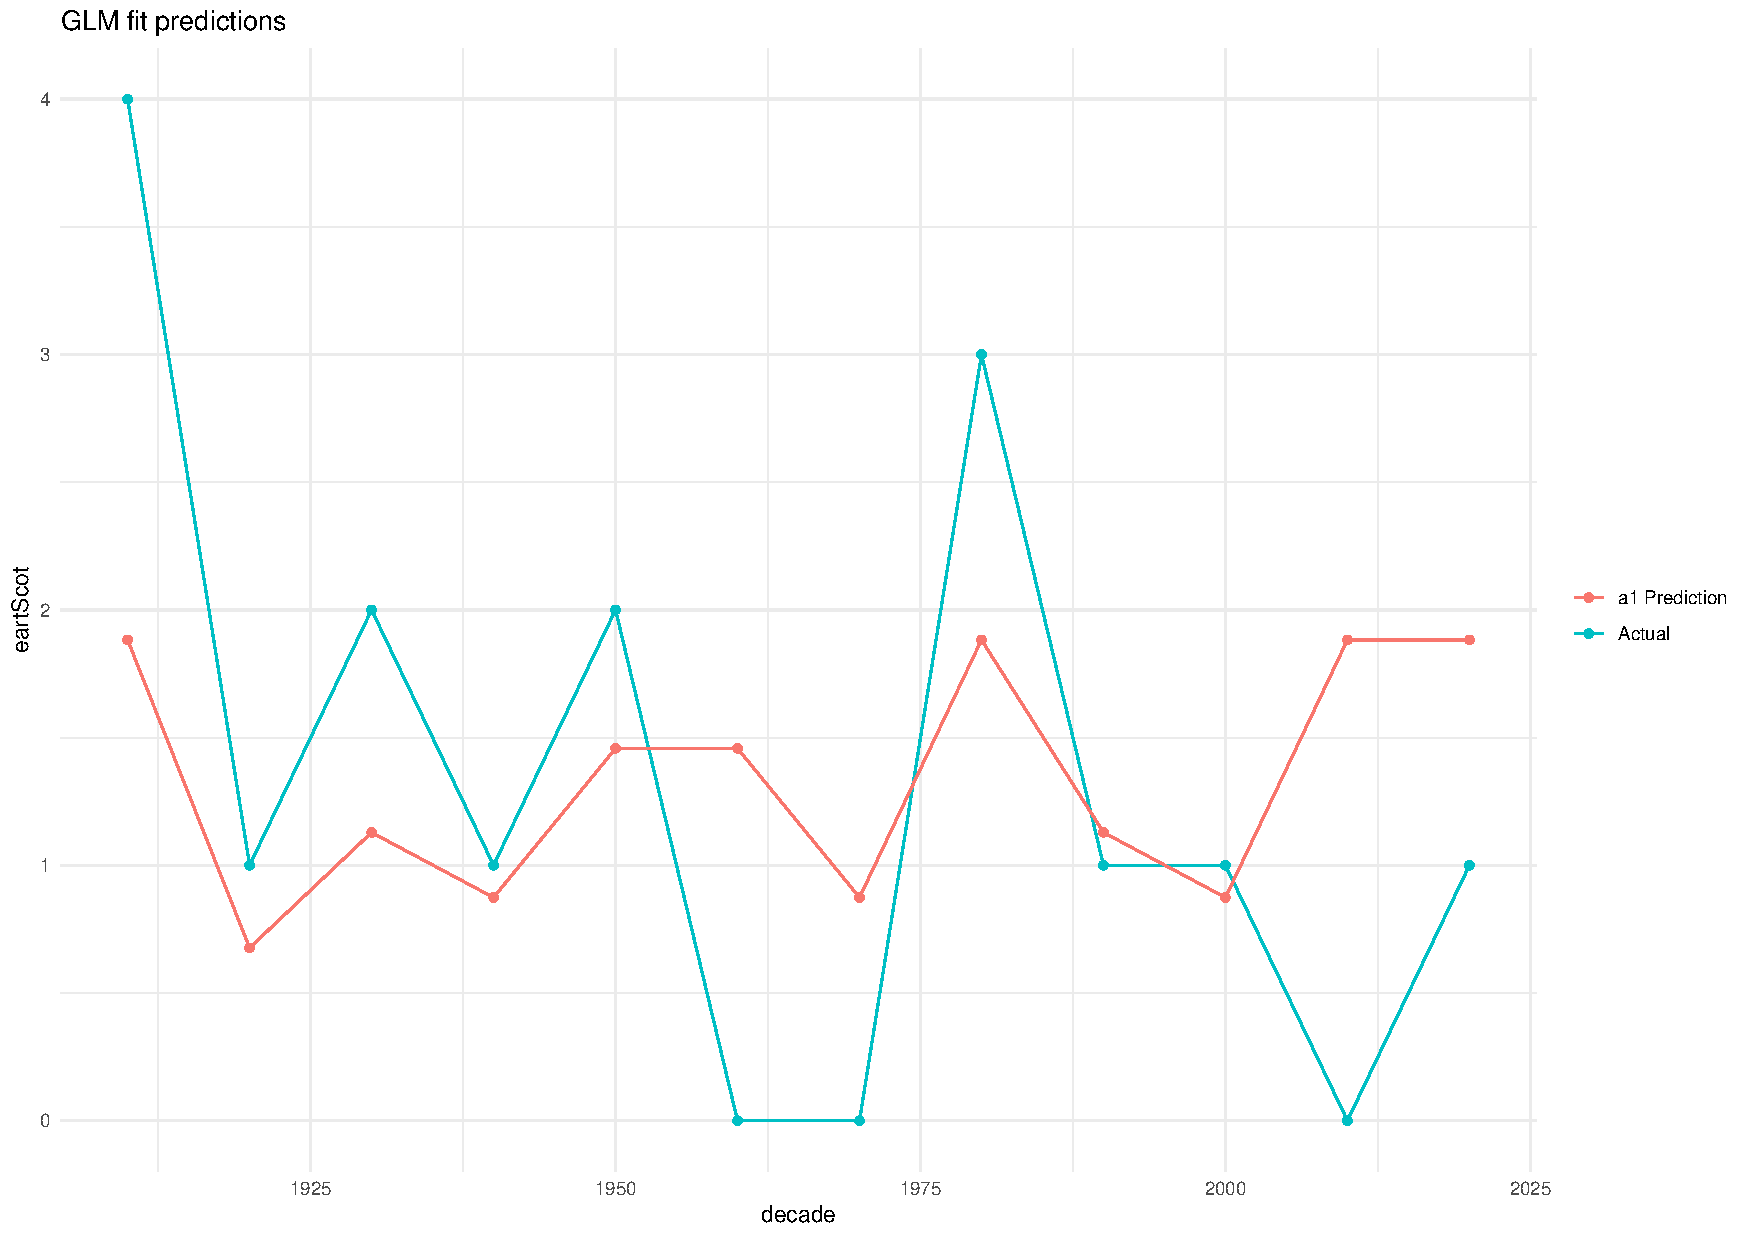
\includegraphics[width=0.6\linewidth]{figures/Rplot02.pdf}
    \caption{Predictions per decade}
    \label{prediction1}
\end{figure}

In \autoref{model1}, the fitted model is plotted, along with 1 standard deviation (the grey area). We can clearly see that the fit is capturing most of the information, however it might not be flexible enough to predict accurately.  In \autoref{prediction1}, we see the observed and the predicted values per decade. We can observe that even in a simple model as this one, the fitted model predicts correctly within plus or minus one earthquake. However, it is apparent that in order to have a bigger accuracy, a more complex model is needed.


\item
Explanation: In this section, three Bayesian Poisson models using JAGS were used in order to better estimate the earthquakes in Scotland. On the first one, the $\lambda$ parameter was modeled to have a prior distribution of $\lambda \sim Gamma(0.01,0.01)$, on the second one $lambda \sim Gamma(16,20)$ while the third one was chosen to be a hierarchical model with $lambda \sim Gamma(a,b)$, $a \sim Lognormal(\ln(2),\ln(1.64))$ and $b \sim Lognormal(\ln(4),\ln(1.64))$. Those numbers where chosen so that the expected value of  $\lambda$ would be 0.5 and the coefficient of variation of $\lambda$ would also be 0.5.

Results: The way convergence was checked was through the trace plots, the Gelman Rubin statistic and the Autocorelation plots, which are presented in \autoref{trace}, \autoref{Gelman}, and \autoref{acf}.

\begin{figure}[h]
    \centering
    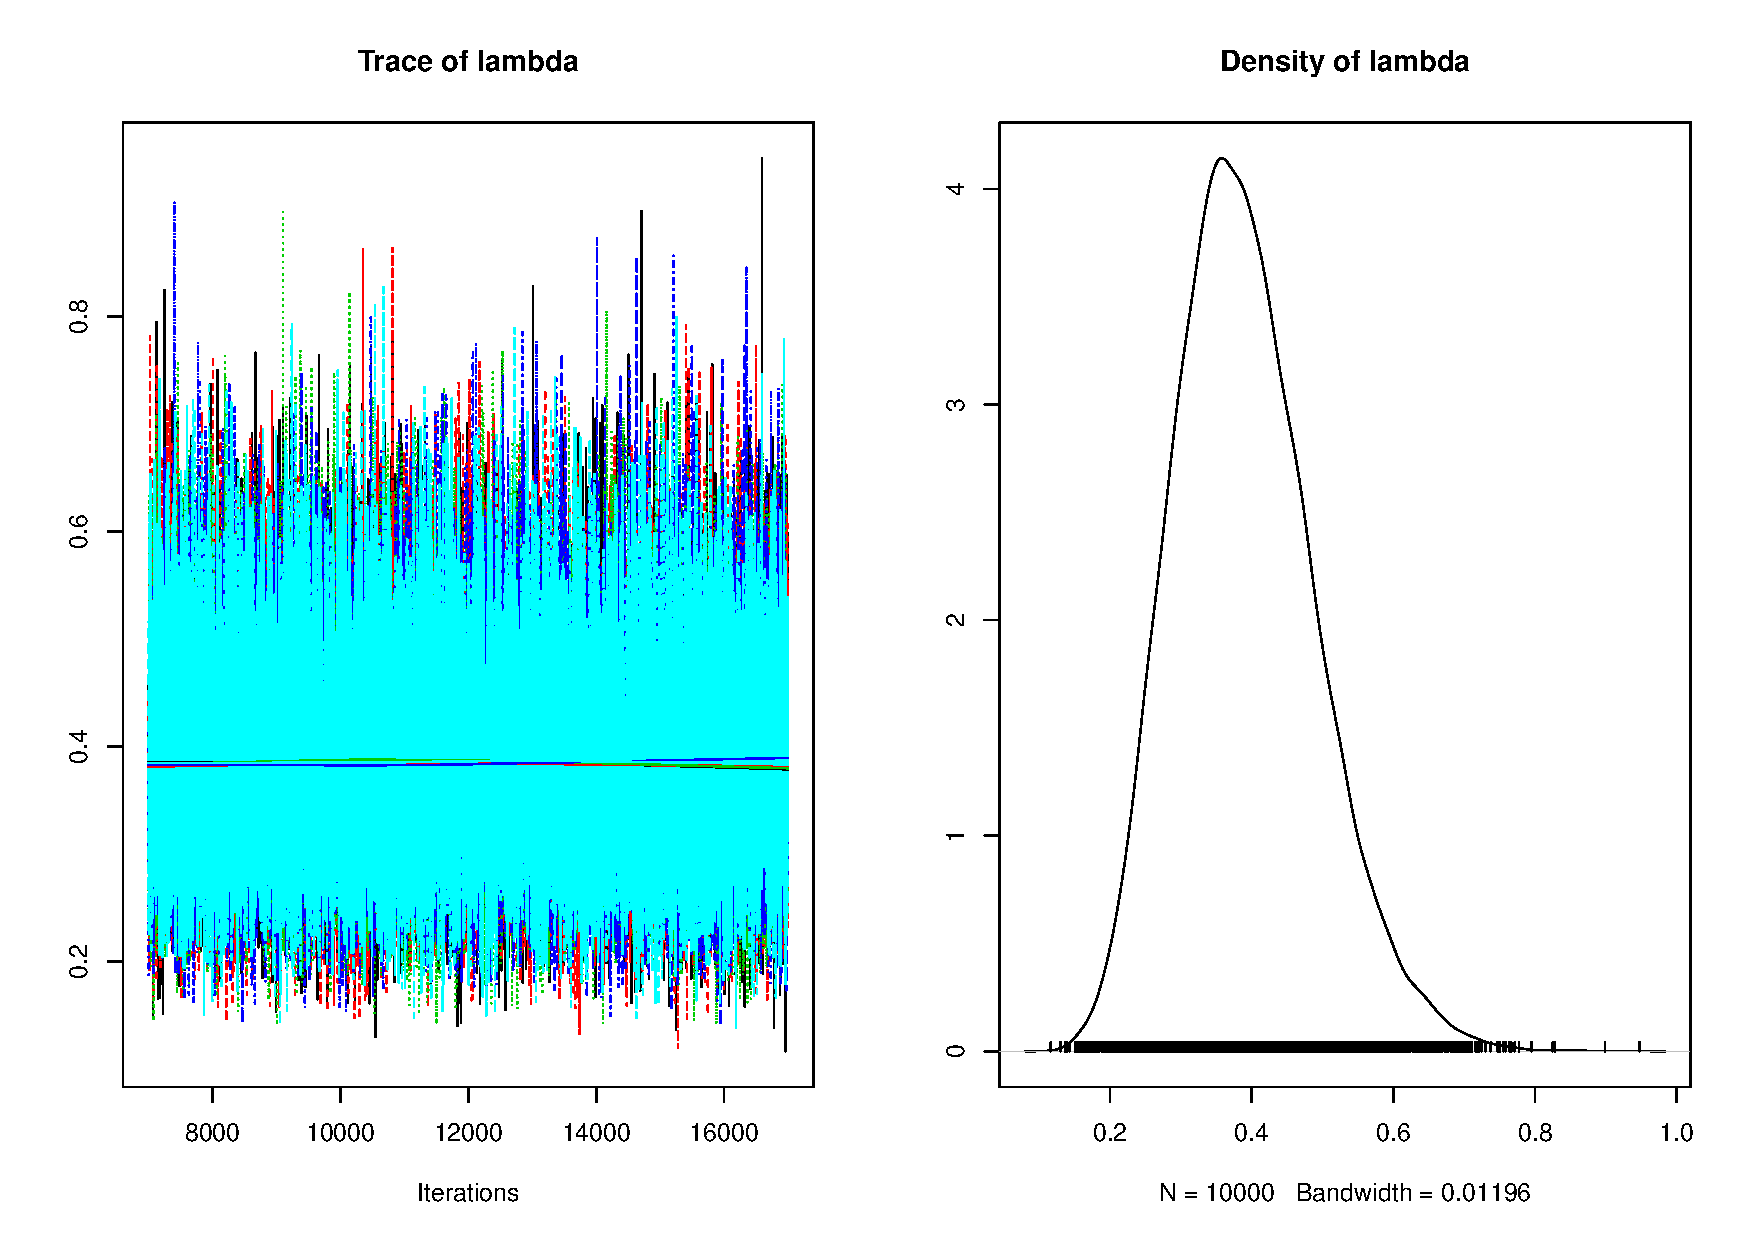
\includegraphics[width=0.6\linewidth]{figures/Rplot03.pdf}
    \caption{Trace plot}
    \label{trace}
\end{figure}

\begin{figure}[h]
    \centering
    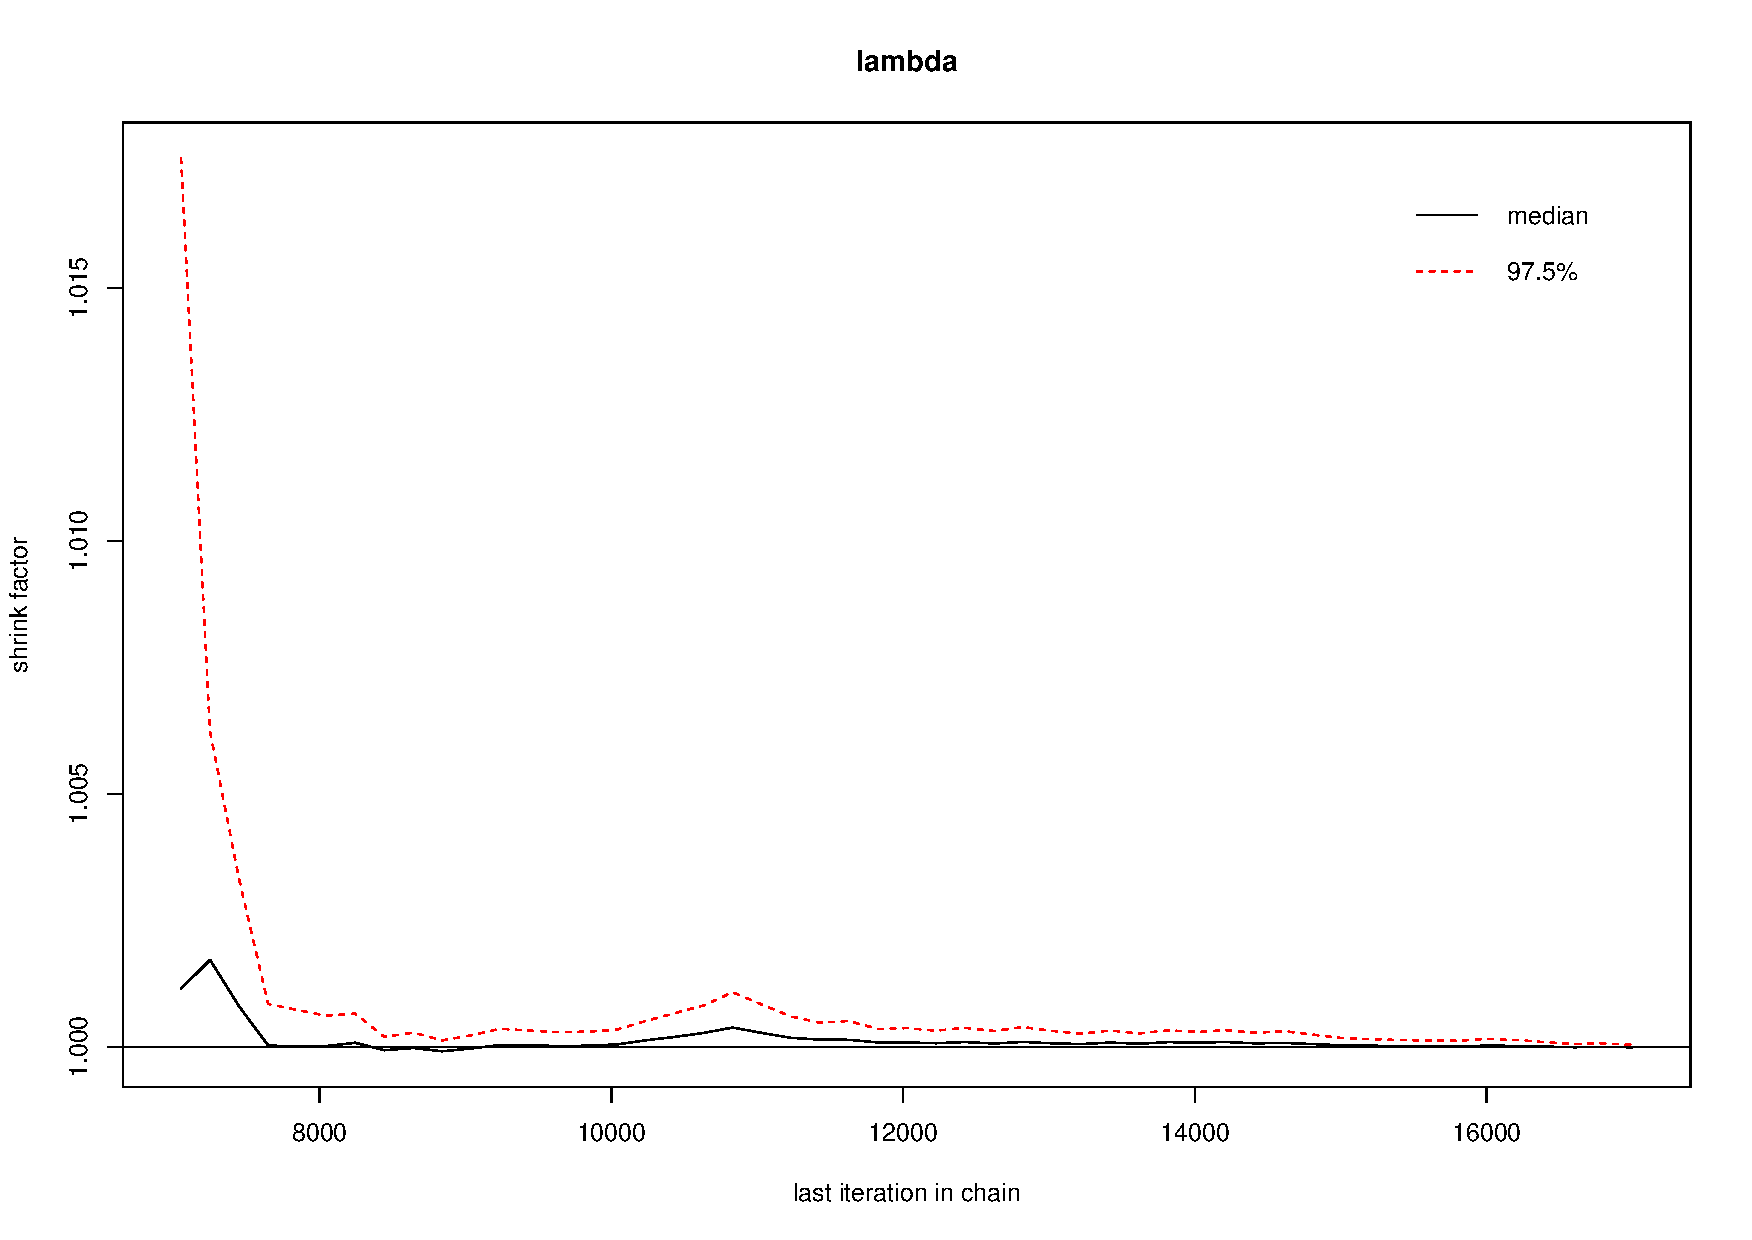
\includegraphics[width=0.6\linewidth]{figures/Rplot04.pdf}
    \caption{Gelman-Rubin plot}
    \label{Gelman}
\end{figure}

\begin{figure}[h]
    \centering
    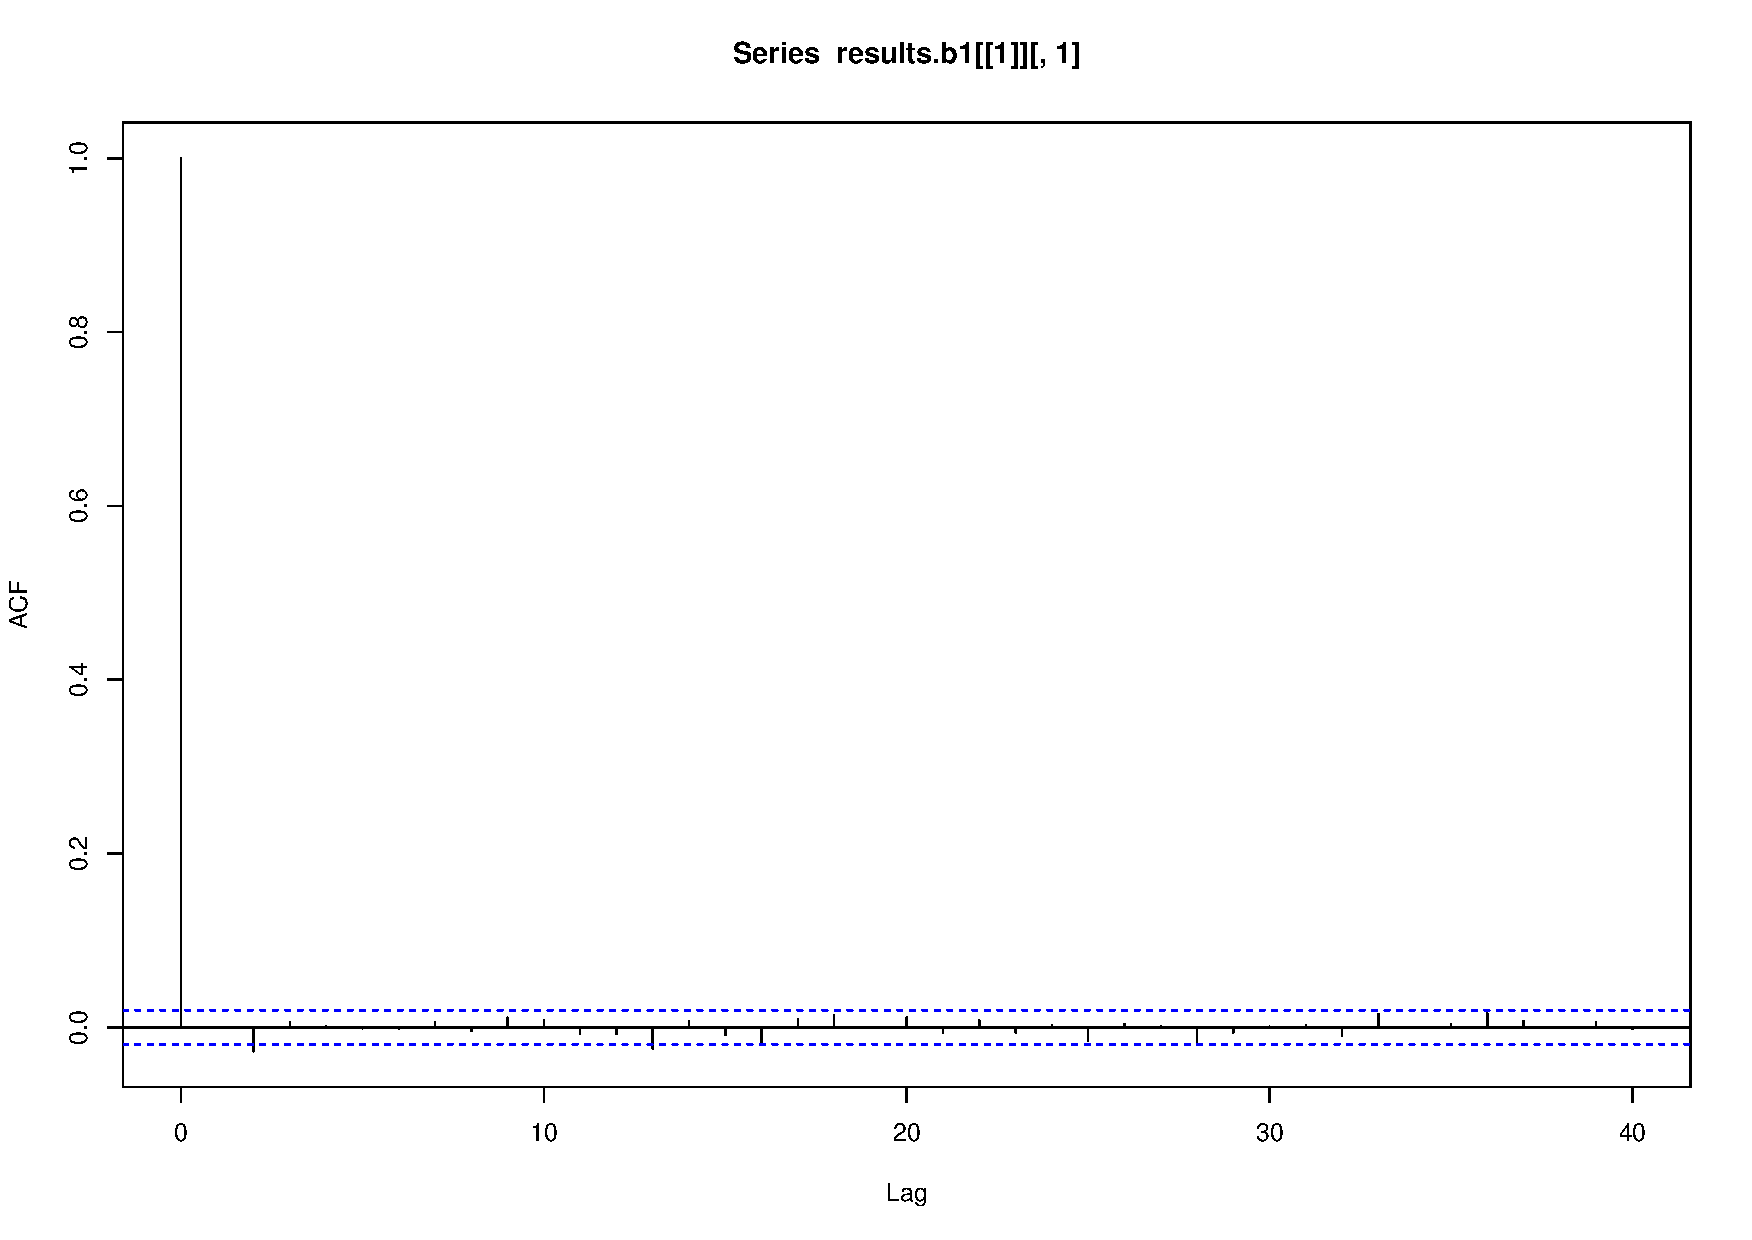
\includegraphics[width=0.6\linewidth]{figures/Rplot05.pdf}
    \caption{ACF plot}
    \label{acf}
\end{figure}

These are the ways all the Markov chain Monte Carlo chains have beed checked for convergence in this assignment.

The results are that 


\item
Explanation:

Results:

\item
Explanation:

Results:

\item
Explanation:

Results:

\end{enumerate}

\noindent\textbf{2)}
\begin{enumerate}[(a)]
\item
Explanation:

Results:

\item
Explanation:

Results:

\item
Explanation:

Results:

\item
Explanation:

Results:

\item
Explanation:

Results:


\end{enumerate}
\end{document}